\documentclass[utf8]{beamer}

%% === CJK 套件 ===
\usepackage{CJKutf8,CJKnumb}                 % 中文套件
%% === AMS 標準套件 ===
\usepackage{amsmath,amsfonts,amssymb,amsthm} % 數學符號
\usepackage{ulem}
%% === TikZ 套件 ===
\usepackage{tikz,tkz-graph,tkz-berge}        % 繪圖
\usepackage{multicol}
\usepackage{xkeyval,xargs}
\usepackage{xcolor}
%% === 插圖套件 ===
\usepackage{caption}
\usepackage{subfigure}

\usetheme{Madrid}
\usecolortheme{crane}

\setbeamertemplate{items}[circle]

\begin{document}
\begin{CJK}{UTF8}{bkai}

\newcommand\MahjongSize{.25}
% == 字牌 ==
%% === 風牌 ===
\providecommand*\Dong{
\includegraphics[scale=\MahjongSize]{./tiles/wind_1_dong.png}}
\providecommand*\Nan{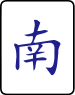
\includegraphics[scale=\MahjongSize]{./tiles/wind_2_nan.png}}
\renewcommand*\Xi{
\includegraphics[scale=\MahjongSize]{./tiles/wind_3_xi.png}}
\providecommand*\Bei{
\includegraphics[scale=\MahjongSize]{./tiles/wind_4_bei.png}}
%% === 三元牌 ===
\providecommand*\Zhong{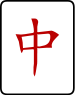
\includegraphics[scale=\MahjongSize]{./tiles/dragon_1_zhong.png}}
\providecommand*\Fa{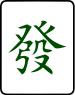
\includegraphics[scale=\MahjongSize]{./tiles/dragon_2_fa.png}}
\providecommand*\Bai{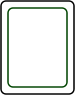
\includegraphics[scale=\MahjongSize]{./tiles/dragon_3_bai.png}}
% == 數字牌 ==
\providecommand*\WanTile[1]{\includegraphics[scale=\MahjongSize]{./tiles/wan_#1.png}}
\providecommand*\TongTile[1]{\includegraphics[scale=\MahjongSize]{./tiles/tong_#1.png}}
\providecommand*\TiaoTile[1]{\includegraphics[scale=\MahjongSize]{./tiles/tiao_#1.png}}
% == 牌背 ==
\providecommand*\Back{
\includegraphics[scale=\MahjongSize]{./tiles/back.png}}
% == 集合 ==
\providecommand*\Wind{\Dong\Nan\Xi\Bei}
\providecommand*\Dragon{\Zhong\Fa\Bai}
\providecommand*\Zhi{\Wind\Dragon}
\providecommand*\Wan{\WanTile{1}\WanTile{2}\WanTile{3}\WanTile{4}\WanTile{5}\WanTile{6}\WanTile{7}\WanTile{8}\WanTile{9}}
\providecommand*\Tong{\TongTile{1}\TongTile{2}\TongTile{3}\TongTile{4}\TongTile{5}\TongTile{6}\TongTile{7}\TongTile{8}\TongTile{9}}
\providecommand*\Tiao{\TiaoTile{1}\TiaoTile{2}\TiaoTile{3}\TiaoTile{4}\TiaoTile{5}\TiaoTile{6}\TiaoTile{7}\TiaoTile{8}\TiaoTile{9}}
\providecommand*\OldMan{\WanTile{1}\WanTile{9}\TongTile{1}\TongTile{9}\TiaoTile{1}\TiaoTile{9}}
\providecommand*\OneNine{\OldMan\Zhi}
% == 牌搭 ==
\providecommand*\DarkGang[1]{%
  \begin{subfigure}{}
    {#1}\Back\Back{#1}
  \end{subfigure}}


\title{從臺灣麻將簡介日本麻將}
\author{開源麻將少女}

\begin{frame}
  \titlepage
\end{frame}
\begin{frame}
  \frametitle{大綱}
  \begin{multicols}{2}
    \tableofcontents
  \end{multicols}
\end{frame}

\section{基礎介紹}
\begin{frame}
  \frametitle{大綱}
  \begin{multicols}{2}
    \tableofcontents[currentsection]
  \end{multicols}
\end{frame}

\subsection{簡介}
\begin{frame}
  \frametitle{與臺灣麻將的差異}
  \begin{alertblock}{差異}
    \begin{enumerate}
    \item 13 張麻將:與臺麻 16 張不同
    \item 排名麻將:會先約定打\alert{東風場}或\alert{東南場},每局麻將結束用\alert{點數}計分,整場結束後依照點數多寡計算排名。
    \item 一台起和:沒有屁胡。
    \item 牌數、類型不同:不使用花牌,有紅寶牌。
    \item 棄牌要排好,一排六個。
    \item 叫牌時牌的擺法有特殊規定。
    \end{enumerate}
  \end{alertblock}
\end{frame}

\subsection{牌種}
\begin{frame}
  \frametitle{牌種}
  \begin{enumerate}
  \item 字牌,共七種。又可分為兩類:
    \begin{itemize}
    \item 風牌:\Wind
    \item 三元牌:\Dragon
    \end{itemize}
  \item 萬字牌,共九種:\Wan
  \item 筒子牌,共九種:\Tong
  \item 條子牌,共九種:\Tiao
  \end{enumerate}
\end{frame}

\begin{frame}
  \frametitle{特殊牌類}
  \begin{itemize}
  \item \alert{老頭牌},數字牌的 1 和 9:\OldMan
  \item \alert{么九牌},老頭牌+字牌:
    \begin{figure}
    \centering
    \OneNine
    \end{figure}
  \item \alert{紅寶牌}:紅色的五萬、五筒、五條。
  \end{itemize}
\end{frame}

\subsection{番數與役種}
\begin{frame}
  \frametitle{番數與役種}
  \begin{exampleblock}{番數}
    \begin{itemize}
    \item 可以看作是臺灣麻將的「台數」。
    \item 不同番數有不同的稱呼,會和\alert{點數的計算}有關。
      \begin{table}
        \begin{tabular}{|c|c|}
        \hline
        稱呼 & 番數\\
        \hline
        \hline
        滿貫 & 3 至 5 番\\
        \hline
        跳滿 & 6 至 7 番\\
        \hline
        倍滿 & 8 至 10 番\\
        \hline
        三倍滿 & 11 至 12 番\\
        \hline
        役滿 或 累計役滿 & 13 番以上\\
        \hline
        \end{tabular}
      \end{table}
    \item 備註:只有\alert{部分}情況才有滿貫,後面算分會說明。
    \end{itemize}
  \end{exampleblock}
  \begin{alertblock}{役種}
    \begin{itemize}
    \item 就是「和牌牌型」,有三暗刻、四暗刻、一盃口等等。
    \end{itemize}
  \end{alertblock}
\end{frame}

\subsection{點棒與立直}

\begin{frame}
  \frametitle{點棒}
  \begin{block}{點棒}
    \begin{itemize}
    \item 日本麻將的點數,有一百點、一千點、五千點、一萬點四種。
    \item 開局時,每人 25000 點;若是三人麻將,開局每人 35000 點。
    \end{itemize}
  \end{block}
\end{frame}

\begin{frame}
  \frametitle{立直}
  \begin{block}{立直}
    \begin{itemize}
      \item \alert{門清}時聽牌可選擇「叫聽」,此時丟出 1000 點做為代價。
      \item 因為日本麻將沒番不可和,因此立直算一番 (一台),就可以和牌。
      \item 立直發動後,\alert{不可以換張},只能摸打、和別人牌或自摸。
    \end{itemize}
  \end{block}
  \begin{exampleblock}{註}
    \begin{itemize}
    \item 是日麻高分常見手段,因為很多牌型都需要\alert{門清}。
    \item 如果別人和牌,先前丟出去的 1000 點歸和牌者所有。
    \item 流局則累積到下一場。
    \end{itemize}
  \end{exampleblock}
\end{frame}

\begin{frame}
  \frametitle{與臺灣麻將的差異}
\end{frame}

\section{和牌役種}
\subsection{順子役與刻子役}
\begin{frame}
  \frametitle{大綱}
  \begin{multicols}{2}
    \tableofcontents[currentsection,currentsubsection]
  \end{multicols}
\end{frame}

\begin{frame}
  \frametitle{順子役}
  \begin{block}{一番役}
    \begin{itemize}
    \item 一盃口:相同花色的兩組順子。
      \begin{figure}
        \centering
        \WanTile{1}\WanTile{1}\WanTile{2}\WanTile{2}\WanTile{3}\WanTile{3}
      \end{figure}
    \item 平胡:只有順子、客風牌,且兩面聽和牌。
      \begin{figure}
        \centering
        \WanTile{4}\WanTile{5}\WanTile{6}\TongTile{5}\TongTile{6}\TongTile{7}\TongTile{8}\TongTile{9}\TiaoTile{2}\TiaoTile{3}\TiaoTile{4}\Dong\Dong{槍和}\TongTile{7}
      \end{figure}
    \end{itemize}
  \end{block}
\end{frame}

\begin{frame}
  \frametitle{順子役}
  \begin{block}{二番役}
    \begin{itemize}
    \item 一氣通貫:同花色 1 到 9。
      \begin{figure}
        \centering
        \Tong\TiaoTile{4}\TiaoTile{4}\TiaoTile{4}\Xi自摸\Xi
      \end{figure}
    \item 三色同順:萬、筒、條三種花色有相同順子。
      \begin{figure}
        \centering
        \WanTile{5}\WanTile{6}\WanTile{6}\WanTile{6}\WanTile{7}\TongTile{5}\TongTile{7}\TiaoTile{5}\TiaoTile{6}\TiaoTile{7}\Nan\Nan\Nan{槍和}\TongTile{6}
      \end{figure}
    \end{itemize}
  \end{block}
\end{frame}

\begin{frame}
  \frametitle{順子役}
  \begin{alertblock}{三番役}
    \begin{itemize}
    \item 二盃口:兩組一盃口,\alert{非門前清不能和}。(和牌不計一盃口)
      \begin{figure}
        \centering
        \WanTile{2}\WanTile{2}\WanTile{3}\WanTile{3}\WanTile{4}\WanTile{4}\TiaoTile{1}\TiaoTile{1}\TiaoTile{2}\TiaoTile{2}\TiaoTile{3}\TiaoTile{3}\Fa{自摸}\Fa
      \end{figure}
    \end{itemize}
  \end{alertblock}
  \begin{exampleblock}{特色}
    \begin{itemize}
    \item 除了二盃口和牌要求門前清外,其他和牌\alert{非門前清時少一番}。
    \item 也就是說一番役在非門前清時\alert{不計}。
    \end{itemize}
  \end{exampleblock}
\end{frame}

\begin{frame}
  \frametitle{刻子役}
  \begin{block}{二番役}
    \begin{itemize}
    \item 對對和:全部由刻子組成。
    \item 三暗刻:和牌有三組暗刻。
    \item 三色同刻:萬、筒、條有相同數字的刻子。
    \item 三槓子:三個槓子。
    \end{itemize}
  \end{block}
\end{frame}

\subsection{么九役與顏色役}
\begin{frame}
  \frametitle{大綱}
  \begin{multicols}{2}
    \tableofcontents[currentsection,currentsubsection]
  \end{multicols}
\end{frame}

\begin{frame}
  \frametitle{么九役}
  \begin{block}{么九役}
    \begin{itemize}
    \item 斷么九(一番)
    \item 混全帶么九(二番)
    \item 純全帶么九(三番)
    \item 混老頭(三番)
    \end{itemize}
  \end{block}
\end{frame}

\begin{frame}
  \frametitle{顏色役}
  \begin{block}{顏色役}
    \begin{itemize}
    \item 混一色(三番)
    \item 清一色(六番)
    \end{itemize}
  \end{block}
\end{frame}

\begin{frame}
  \frametitle{機會役}
  \begin{block}{機會役}
    \begin{itemize}
    \item 門前清自摸和
    \item 搶槓
    \item 嶺上開花
    \item 海底撈月
    \item 河底撈魚
    \end{itemize}
  \end{block}
\end{frame}

\subsection{特殊役}
\begin{frame}
  \frametitle{大綱}
  \begin{multicols}{2}
    \tableofcontents[currentsection,currentsubsection]
  \end{multicols}
\end{frame}

\begin{frame}
  \frametitle{特殊役}
  \begin{block}{一番役}
    \begin{itemize}
    \item 役牌
    \item 立直
    \item 一發
    \end{itemize}
  \end{block}
  \begin{block}{二番役}
    \begin{itemize}
    \item 雙立直
    \item 七對子
    \item 小三元
    \end{itemize}
  \end{block}
\end{frame}

\begin{frame}
  \frametitle{特殊役}
  \begin{exampleblock}{流局滿貫}
  \end{exampleblock}
\end{frame}

\subsection{役滿役}
\begin{frame}
  \frametitle{大綱}
  \begin{multicols}{2}
    \tableofcontents[currentsection,currentsubsection]
  \end{multicols}
\end{frame}

\begin{frame}
  \frametitle{役滿役}
  \begin{itemize}
    \item 天和
    \item 地和
    \item 小四喜
    \item 大三元
    \item 四暗刻
    \item 四槓子
    \item 清老頭
    \item 字一色
    \item 綠一色
    \item 九蓮寶燈
    \item 國士無雙
  \end{itemize}
\end{frame}

\begin{frame}
  \frametitle{雙役滿}
  \begin{itemize}
    \item 大四喜
    \item 四暗刻單騎
    \item 純正九蓮寶燈
    \item 國士無雙十三面
  \end{itemize}
\end{frame}

\subsection{地方役}
\begin{frame}
  \frametitle{大綱}
  \begin{multicols}{2}
    \tableofcontents[currentsection,currentsubsection]
  \end{multicols}
\end{frame}

\begin{frame}
  \frametitle{地方役}
  \begin{block}{地方役}
    \begin{itemize}
    \item 四連刻
    \item 大車輪、大竹林、大數鄰
    \item 加賀百萬石
    \item 紅孔雀
    \item 黑一色
    \item 真似滿
    \item 八連莊
    \end{itemize}
  \end{block}
\end{frame}

\subsection{創作役}
\begin{frame}
  \frametitle{大綱}
  \begin{multicols}{2}
    \tableofcontents[currentsection,currentsubsection]
  \end{multicols}
\end{frame}

\begin{frame}
  \frametitle{創作役}
  \begin{block}{創作役}
    \begin{itemize}
    \item 槍一色:手牌全是槍牌。
    \item 天地創世:白板四暗槓自摸。
      \begin{figure}
      \centering
      \DarkGang{\Bai}\DarkGang{\Bai}\DarkGang{\Bai}\DarkGang{\Bai}\Bai{自摸}\Bai
      \end{figure}
    \end{itemize}
  \end{block}
\end{frame}

\section{計算點數}

\subsection{符數與番數}

\clearpage
\end{CJK}
\end{document}